
%%%%%%%%%%%%%%%%%%%%%%% file typeinst.tex %%%%%%%%%%%%%%%%%%%%%%%%%
%
% This is the LaTeX source for the instructions to authors using
% the LaTeX document class 'llncs.cls' for contributions to
% the Lecture Notes in Computer Sciences series.
% http://www.springer.com/lncs       Springer Heidelberg 2006/05/04
%
% It may be used as a template for your own input - copy it
% to a new file with a new name and use it as the basis
% for your article.
%
% NB: the document class 'llncs' has its own and detailed documentation, see
% ftp://ftp.springer.de/data/pubftp/pub/tex/latex/llncs/latex2e/llncsdoc.pdf
%
%%%%%%%%%%%%%%%%%%%%%%%%%%%%%%%%%%%%%%%%%%%%%%%%%%%%%%%%%%%%%%%%%%%


\documentclass[runningheads,a4paper]{llncs}




\usepackage{amssymb}
\usepackage{cite}
\setcounter{tocdepth}{3}
\usepackage{graphicx}
\usepackage{url}
\usepackage{float}
\usepackage{subfigure}

\urldef{\mailsa}\path|{hossam.faris}@ju.edu.jo| 
\urldef{\mailsc}\path|erika.siebert-cole,}@ju.edu.jo|    
\newcommand{\keywords}[1]{\par\addvspace\baselineskip
\noindent\keywordname\enspace\ignorespaces#1}

\begin{document}

\mainmatter  % start of an individual contribution

% first the title is needed
\title{SMOTE+Ensembles for Bug Prediction}

% a short form should be given in case it is too long for the running head
\titlerunning{Lecture Notes in Computer Science: Authors' Instructions}

% the name(s) of the author(s) follow(s) next
%
% NB: Chinese authors should write their first names(s) in front of
% their surnames. This ensures that the names appear correctly in
% the running heads and the author index.
%
\author{Hossam Faris%
\thanks{King Abdullah II School for Information Technology, The University of Jordan, Amman, Jordan}%
\and  \and }
%
%\authorrunning{Lecture Notes in Computer Science: Authors' Instructions}
% (feature abused for this document to repeat the title also on left hand pages)

% the affiliations are given next; don't give your e-mail address
% unless you accept that it will be published
\institute{The University of Jordan\\
Amman, Jordan\\
\mailsa\\
%\mailsc\\
%\url{http://www.springer.com/lncs}}
}
%
% NB: a more complex sample for affiliations and the mapping to the
% corresponding authors can be found in the file "llncs.dem"
% (search for the string "\mainmatter" where a contribution starts).
% "llncs.dem" accompanies the document class "llncs.cls".
%

\toctitle{Lecture Notes in Computer Science}
%\tocauthor{Authors' Instructions}
\maketitle


\begin{abstract}
\keywords{}
\end{abstract}


\section{Introduction}



\section{Ensemble classifiers}
\label{ensembles}

\subsection{Random Forests (RF)}
\subsection{Bagging}
\subsection{AdaBoost}

\section{Synthetic minority over-sampling technique (SMOTE)}

SMOTE is an oversampling technique what was first proposed in \cite{chawla2002smote}. This oversampling technique modifies the class distribution in the dataset by oversampling the minority class by creating synthetic samples rather than oversampling with replacement. Synthetic samples are generated by operating in feature space.
The minority class is oversampled by taking out each sample and creating synthetic samples along the line segments that join any/all of the $k$ minority class nearest neighbours. 

The algorithm starts by choosing $k$ nearest neighbors then synthetic samples
are generated by taking the difference between the feature vector of the sample
under consideration and its nearest neighbor. Then it Multiplies the difference by a random number between 0 and 1, and add it to the feature vector under consideration. Therefore, a random point is selected along the line segment between two specific features. Consequently, SMOTE broadens the data region of the minority class examples and forces the decision region of the lass to become more general.



\section{Datasets Description}
\label{data}

CM1: NASA spacecraft instrument
JM1: Real-time predictive ground system: Uses simulations to generate predictions
KC1: Storage management for receiving and processing ground
data
PC3: Flight software for earth orbiting satellite metadata


\section{Model evaluation}
\label{evaluation_criteria}
In order to evalute the performance of the software faults prediction model, we used the confusion matrix that shown in Figure \ref{fig:confusion}, which is a table that is often used to describe the classfication model results. 

\begin{figure}[h]
\label{fig:ss}
\begin{center}
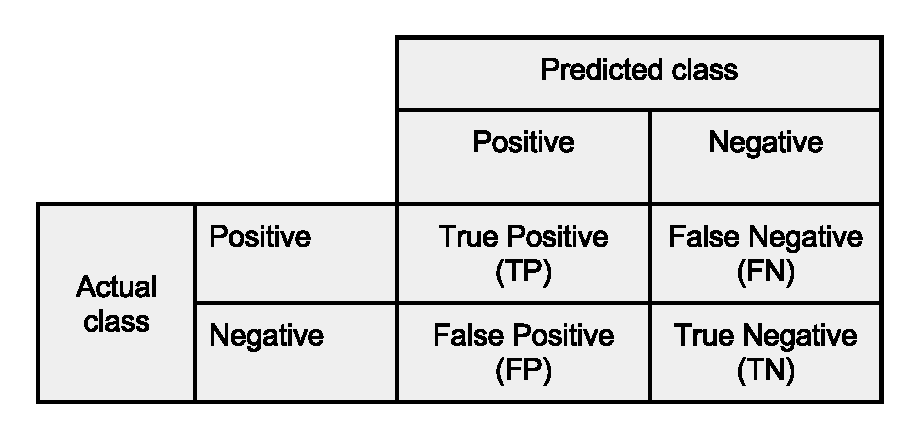
\includegraphics[scale=0.5]{confusion-matrix.eps}
\caption{Confusion matrix}
\end{center}
\label{fig:confusion}
\end{figure}

The bug detection effectiveness is evaluated using four measurements based on the previous confusion matrix; namely, Model Accuracy (Acc), Number of Predicted Defects (PD), Numebr of Incorectly Predicted cases with No Defects (PF), G-mean. Acc is the ratio of the correctly predicted faults to the total number of faults. PD is
the ratio of correctly predicted faults to the total number of faults. PF is the number of not fault-prone modules that are predicted incorrectly as defectes. In addtion, we used the G-mean to combine the PD and PF which is a good indicator of the relationship between the two measures. The PD, PF, G-mean are calculated in Equations \ref{accuracy}, \ref{PD}, \ref{PF}, and \ref{gmean}, respectively.

\begin{equation}
Accuracy=\frac{TP+TN}{TP + FN + FP + TN}
\label{accuracy}
\end{equation}

\begin{equation}
PD=\frac{TP}{TP+FN}
\end{equation}

\begin{equation}
PF=\frac{FP}{FP+TN}
\end{equation}

\begin{equation}
G-mean=\sqrt{PD \times (1-PF)}
\end{equation}

%%%%%%%%%%%%%%%%%%%%%%%%%%%%%%%%%%%%%%%%%%%%

%==================================================================
\section{Experiments and Results}
\label{experiments}



 

%%%%%%%%%%%%%%%%%%%%%%%%%%%%%%
\begin{figure*}[http]
	\scalebox{0.75}{
		\begin{tabular}{p{5cm} p{4cm} p{5cm} }
			\centering
			
			%\subfigure[Appendicitis]{\label{fig:a}\includegraphics[scale=0.40]{appendicitis}}& &
			\subfigure[CM1]{\label{fig:a}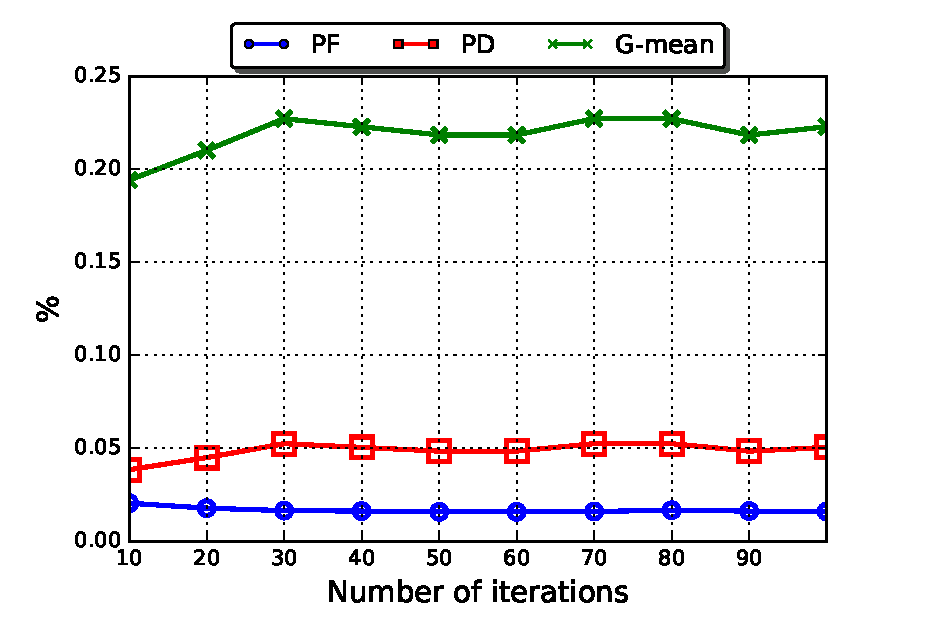
\includegraphics[scale=0.45]{RF-CM1}}& &
			\subfigure[JM1]{\label{fig:a}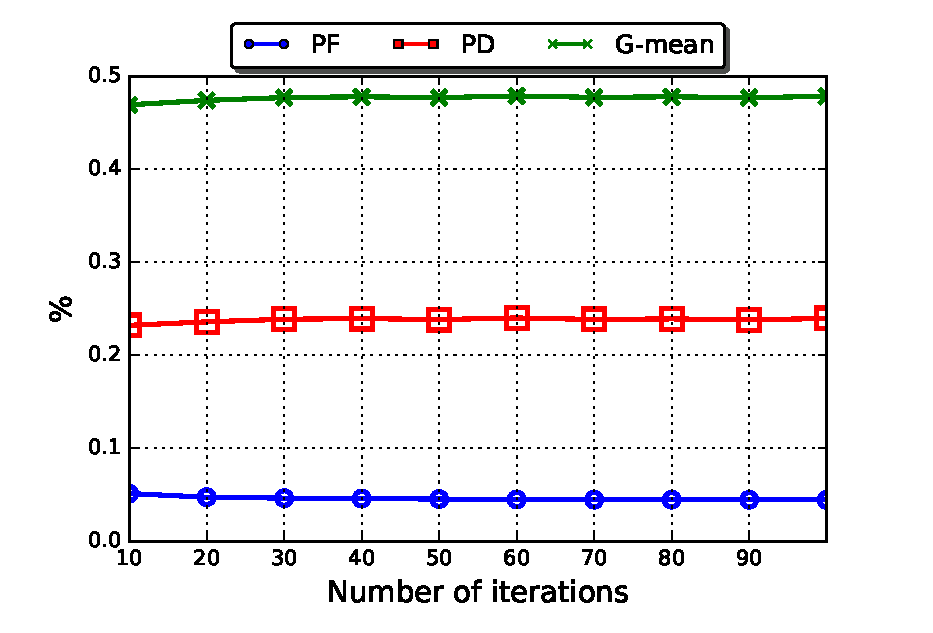
\includegraphics[scale=0.45]{RF-JM1}}

			\vspace{-1.5in}
			\\
			\subfigure[KC1]{\label{fig:a}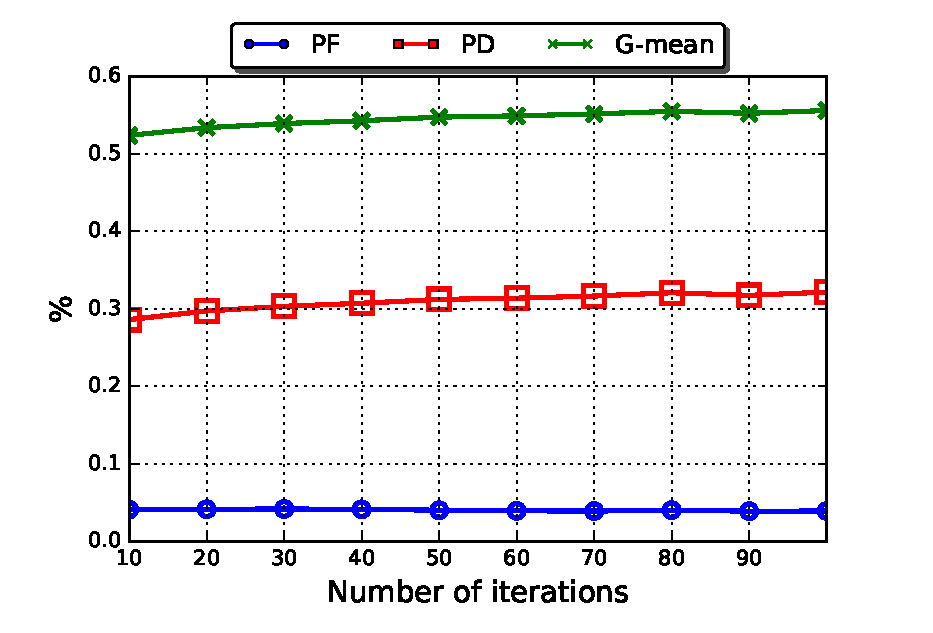
\includegraphics[scale=0.45]{RF-KC1}}& &
			\subfigure[PC3]{\label{fig:a}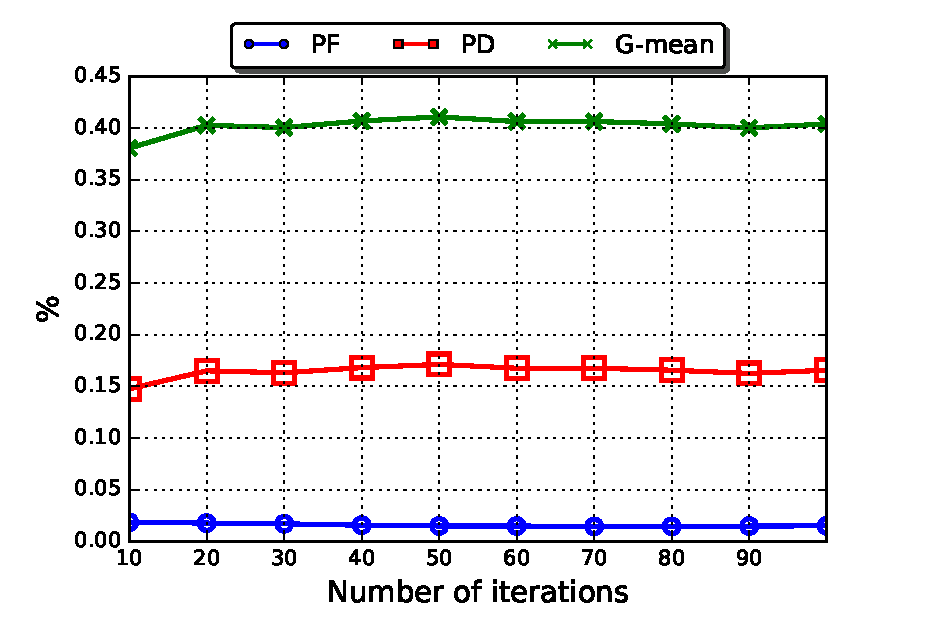
\includegraphics[scale=0.45]{RF-PC3}}

			\vspace{-1.5in}
			\\
%				
		\end{tabular}
	}
	\caption{Evaluation results of RF by changing number of iterations.}
	\label{fig:bestneurons}
	\vspace{-0.0in}
\end{figure*}
%%%%%%%%%%%%%%%%%%%%%%%%%%%%%%%%%%%%%%%%%%%

\begin{figure*}[http]
	\scalebox{0.75}{
		\begin{tabular}{p{5cm} p{4cm} p{5cm} }
			\centering
			
			%\subfigure[Appendicitis]{\label{fig:a}\includegraphics[scale=0.40]{appendicitis}}& &
			\subfigure[CM1]{\label{fig:a}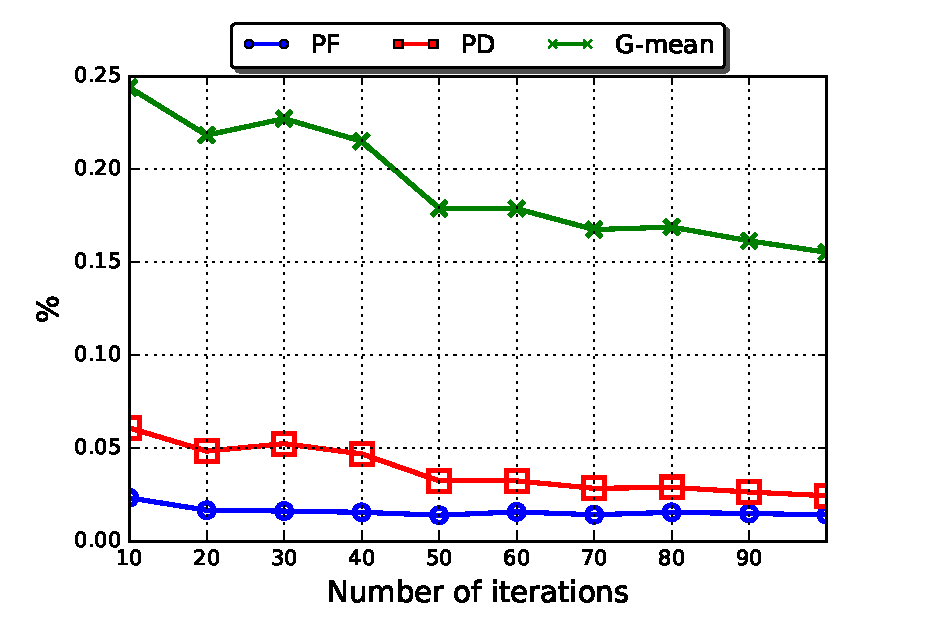
\includegraphics[scale=0.45]{Bagging-CM1}}& &
			\subfigure[JM1]{\label{fig:a}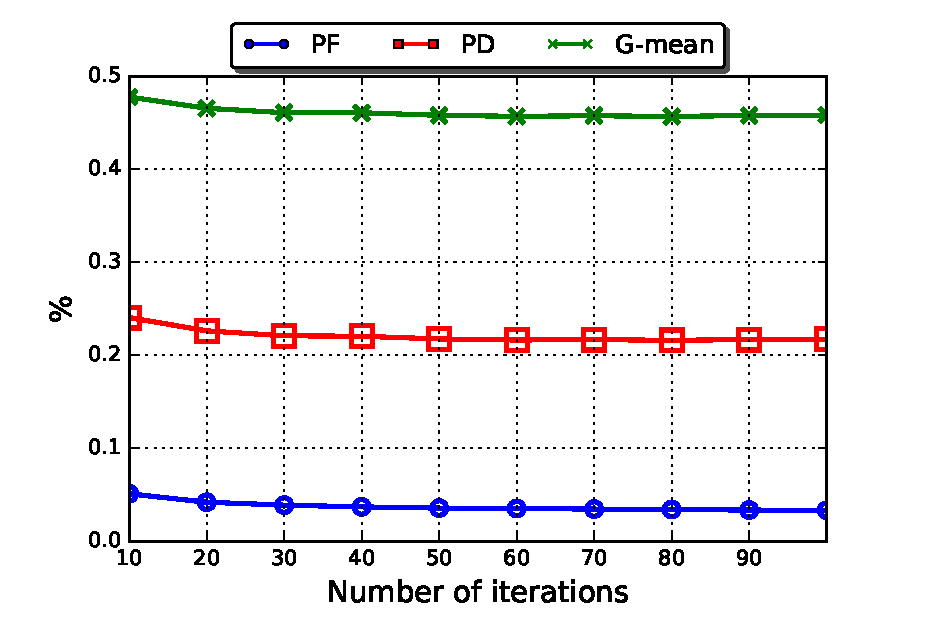
\includegraphics[scale=0.45]{Bagging-JM1}}

			\vspace{-1.5in}
			\\
			\subfigure[KC1]{\label{fig:a}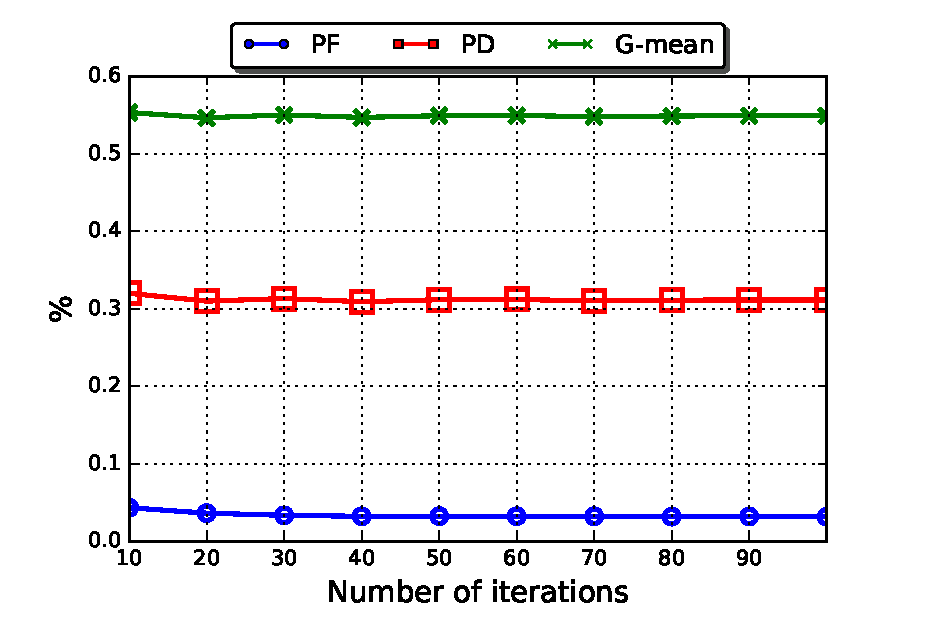
\includegraphics[scale=0.45]{Bagging-KC1}}& &
			\subfigure[PC3]{\label{fig:a}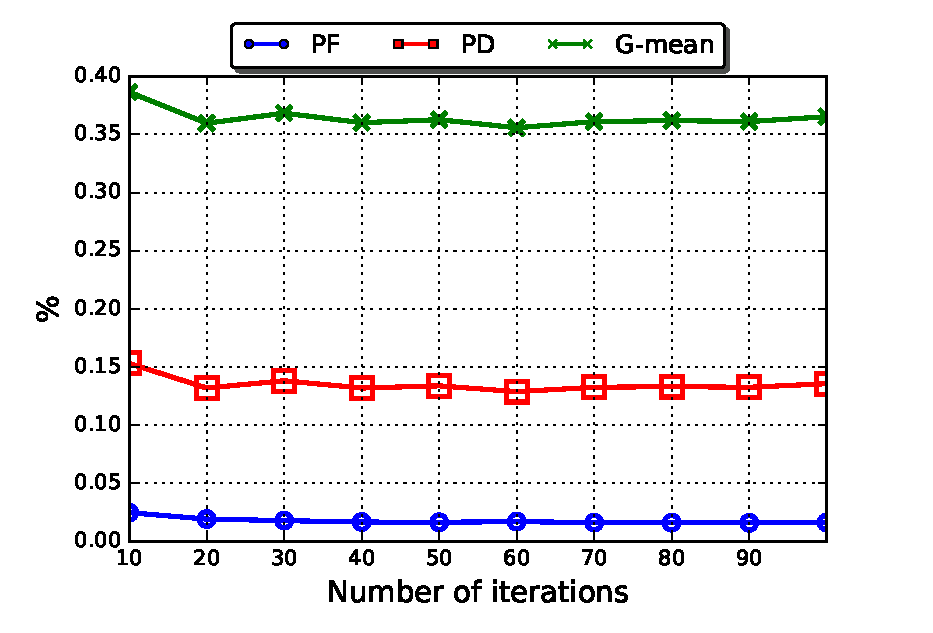
\includegraphics[scale=0.45]{Bagging-PC3}}

			\vspace{-1.5in}
			\\
%				
		\end{tabular}
	}
	\caption{Evaluation results of Bagging by changing number of iterations.}
	\label{fig:bestneurons}
	\vspace{-0.0in}
\end{figure*}
%%%%%%%%%%%%%%%%%%%%%%%%%%%%%%%%%%%%%%%%%%%

\begin{figure*}[http]
	\scalebox{0.75}{
		\begin{tabular}{p{5cm} p{4cm} p{5cm} }
			\centering
			
			%\subfigure[Appendicitis]{\label{fig:a}\includegraphics[scale=0.40]{appendicitis}}& &
			\subfigure[CM1]{\label{fig:a}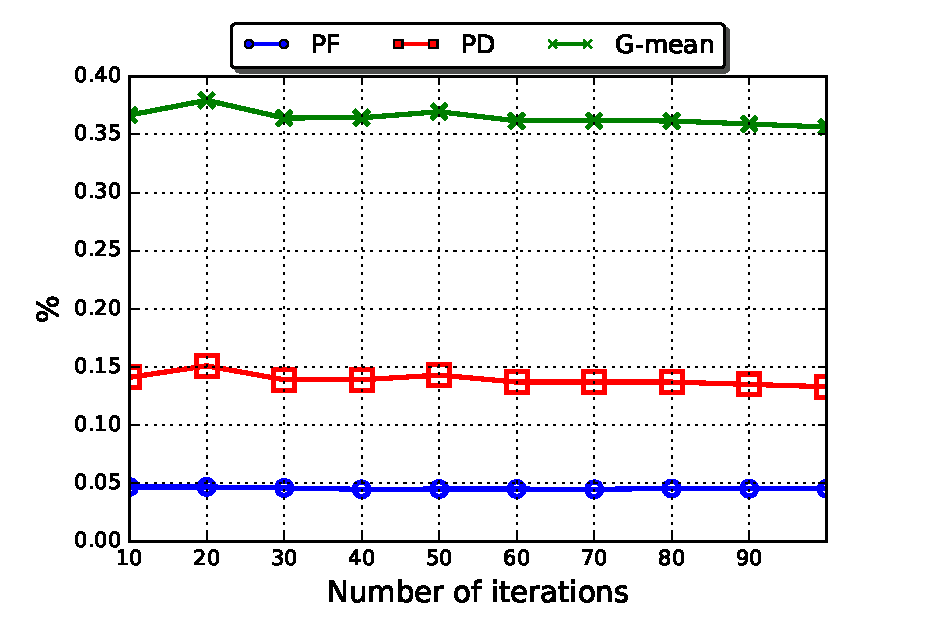
\includegraphics[scale=0.45]{AdaBoost-CM1}}& &
			\subfigure[JM1]{\label{fig:a}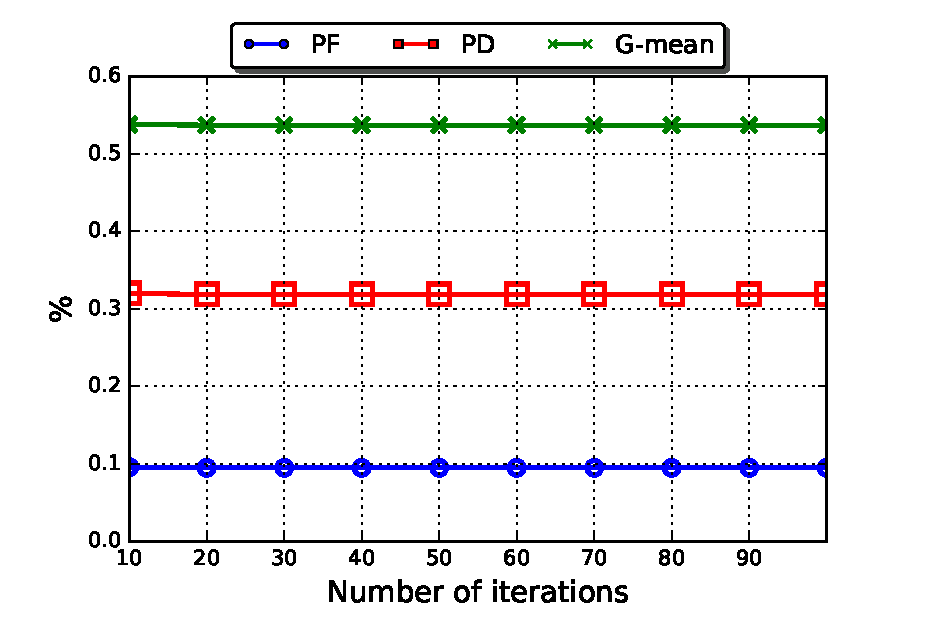
\includegraphics[scale=0.45]{AdaBoost-JM1}}

			\vspace{-1.5in}
			\\
			\subfigure[KC1]{\label{fig:a}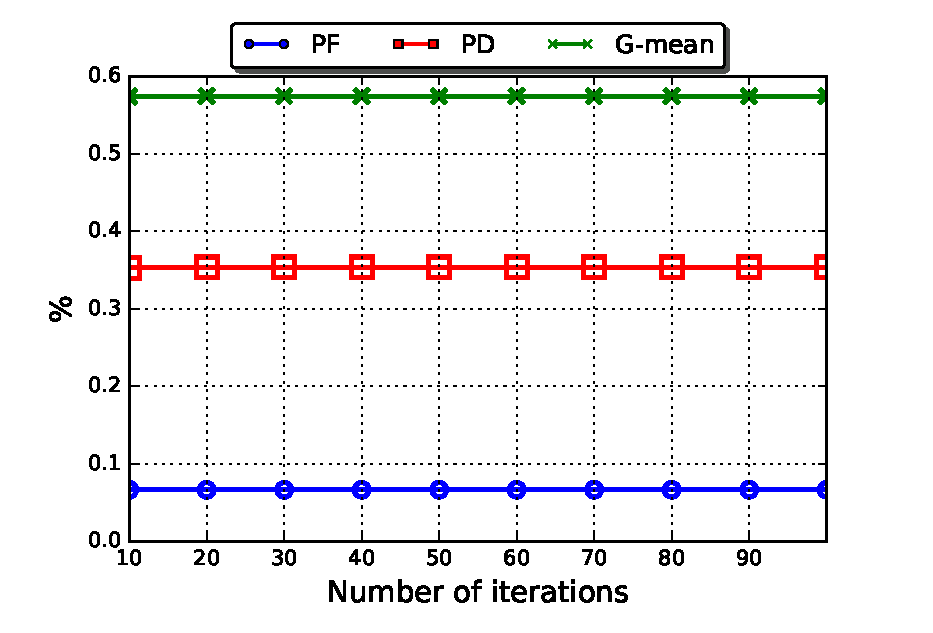
\includegraphics[scale=0.45]{AdaBoost-KC1}}& &
			\subfigure[PC3]{\label{fig:a}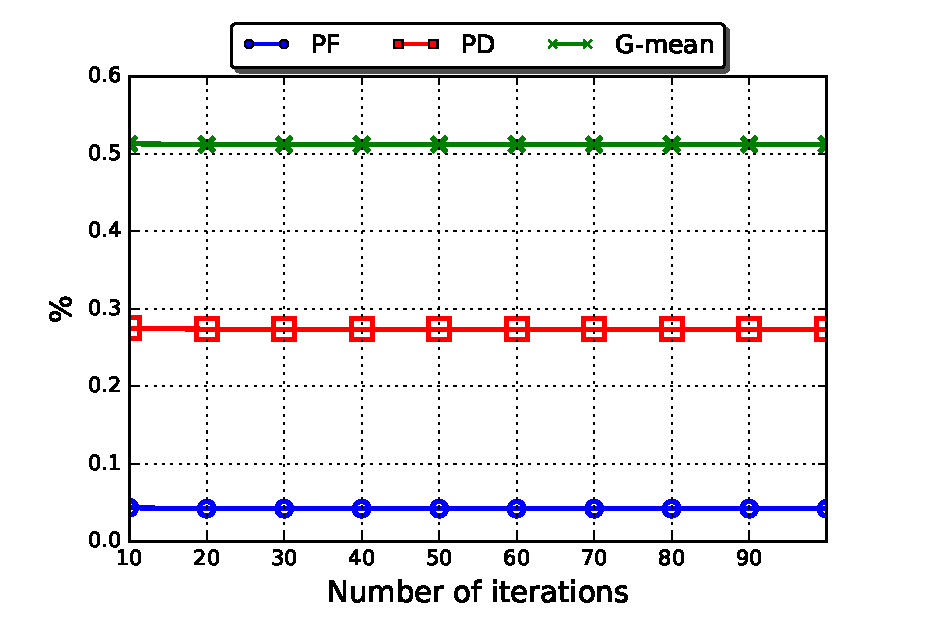
\includegraphics[scale=0.45]{AdaBoost-PC3}}

			\vspace{-1.5in}
			\\
%				
		\end{tabular}
	}
	\caption{Evaluation results of AdaBoost by changing number of iterations.}
	\label{fig:bestneurons}
	\vspace{-0.0in}
\end{figure*}

%%%%%%%%%%%%%%%%%%%%%%%%%%%%%%%%%%%%%%%%%%%

\begin{figure*}[http]
	\scalebox{0.75}{
		\begin{tabular}{p{5cm} p{4cm} p{5cm} }
			\centering
			
			%\subfigure[Appendicitis]{\label{fig:a}\includegraphics[scale=0.40]{appendicitis}}& &
			\subfigure[CM1]{\label{fig:a}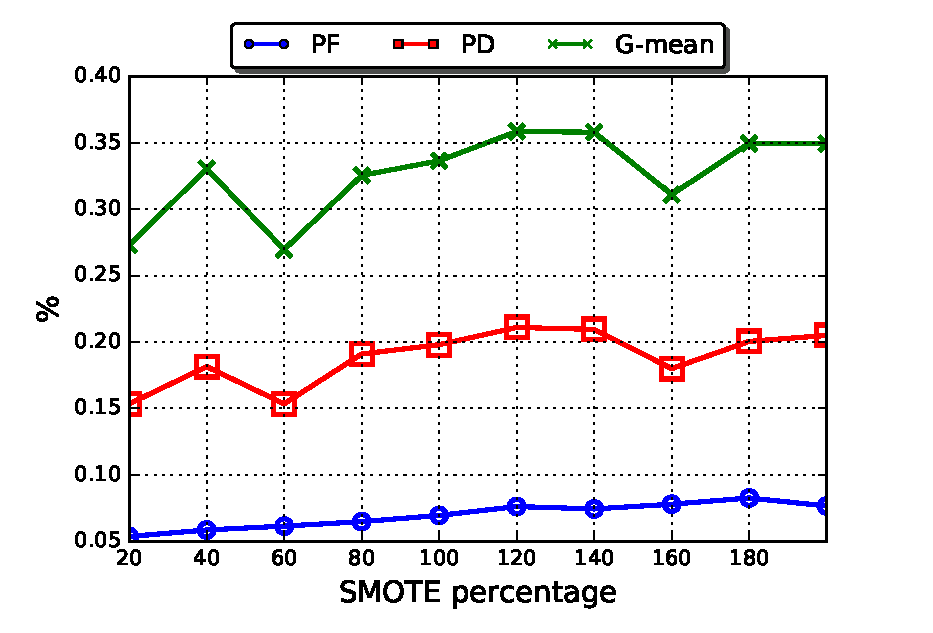
\includegraphics[scale=0.45]{SMOTE-AdaBoost-CM1}}& &
			\subfigure[JM1]{\label{fig:a}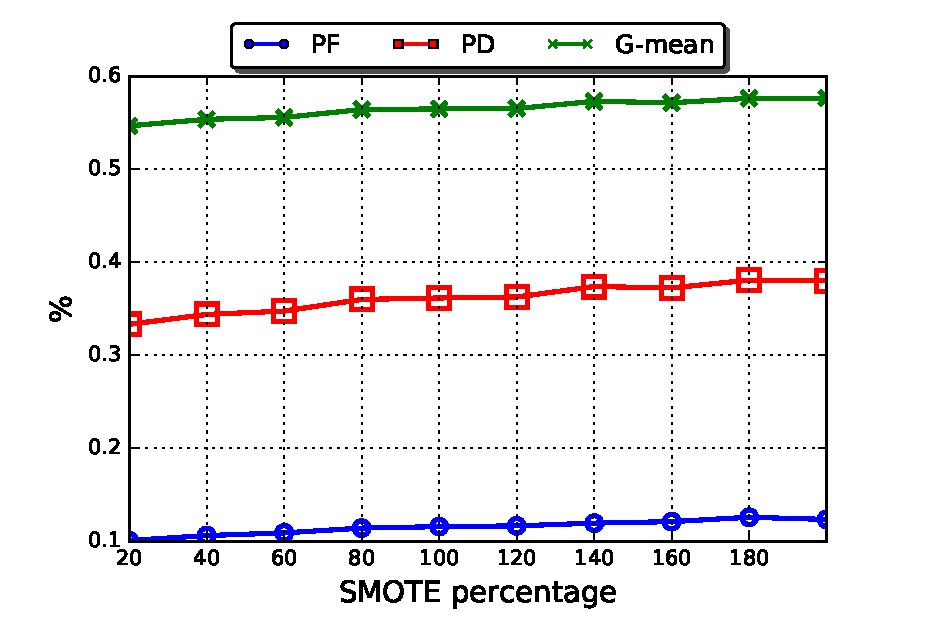
\includegraphics[scale=0.45]{SMOTE-AdaBoost-JM1}}

			\vspace{-1.5in}
			\\
			\subfigure[KC1]{\label{fig:a}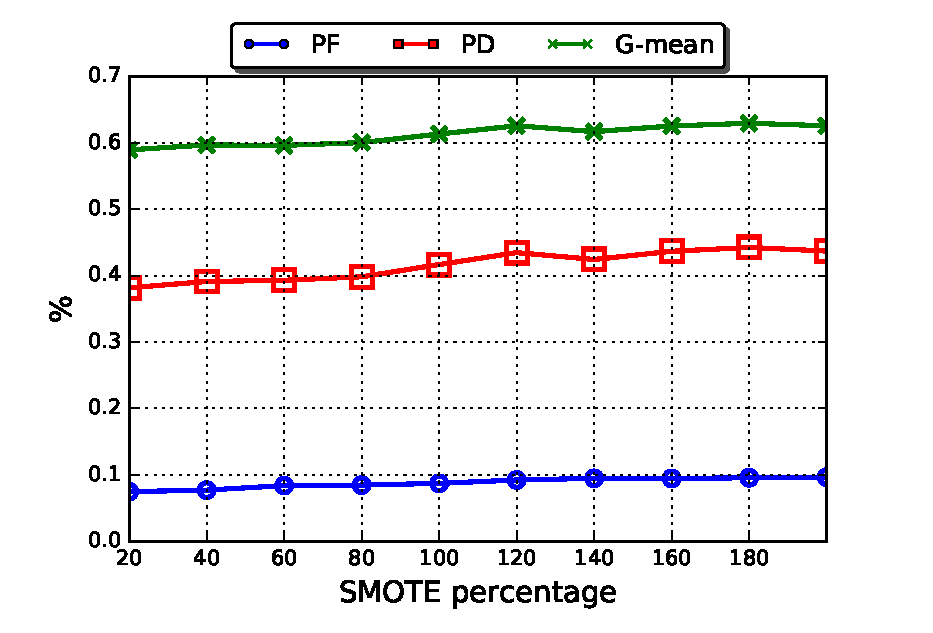
\includegraphics[scale=0.45]{SMOTE-AdaBoost-KC1}}& &
			\subfigure[PC3]{\label{fig:a}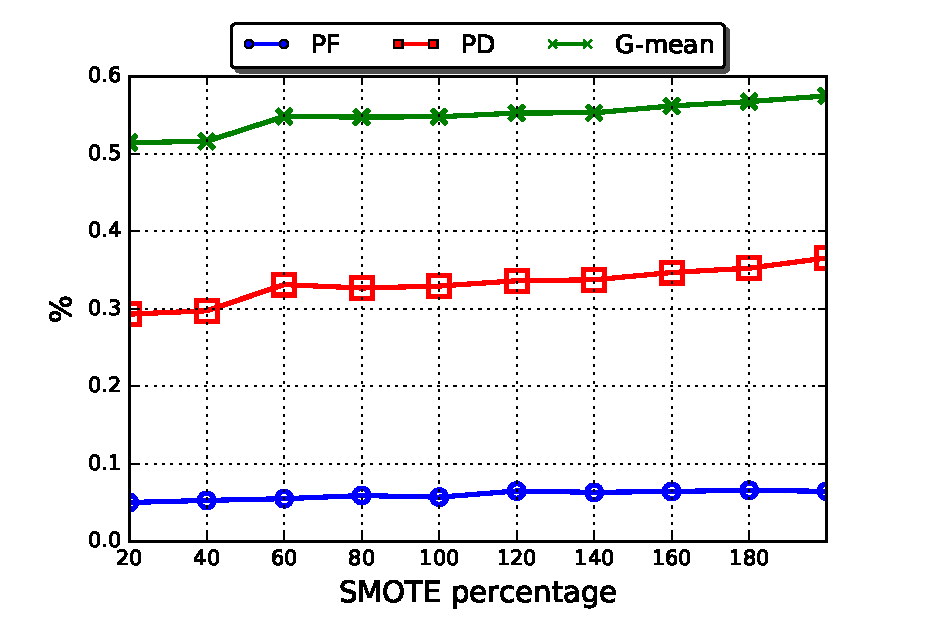
\includegraphics[scale=0.45]{SMOTE-AdaBoost-PC3}}

			\vspace{-1.5in}
			\\
%				
		\end{tabular}
	}
	\caption{Evaluation results of SMOTE+AdaBoost by changing number of iterations.}
	\label{fig:bestneurons}
	\vspace{-0.0in}
\end{figure*}




\section{Conclusions}
\label{conclusion}




%\subsection*{Acknowledgments.} Authors would like to thank the Jordanian mobile telecommunication operator Umniah for providing the required technical assistance and the data for this developed research work.




\bibliographystyle{splncs}
\bibliography{ref}
\end{document}
